  %Real world situation, not bringing in outside subject, system to solve inequality
\begin{center}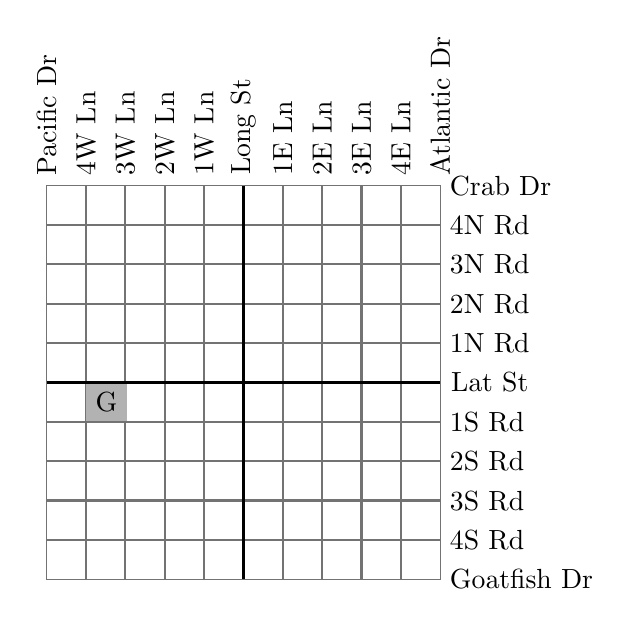
\begin{tikzpicture}[scale=0.5]
\foreach \i in {-4,-3,...,4}{
\draw[thick,black!55](\i,-5)--(\i,5)(-5,\i)--(5,\i);
};
\foreach \i in {1,2,3,4}{
\draw(\i,5)node[rotate=90,anchor=west]{\i E Ln} (-\i,5)node[rotate=90,anchor=west]{\i W Ln} (5,\i)node[anchor=west]{\i N Rd} (5, -\i)node[anchor=west]{\i S Rd};
};
\draw[very thick](-5,0)--(5,0)node[anchor=west]{Lat St} (0,-5)--(0,5)node[anchor=west,rotate=90]{Long St};
\draw[black!55](-5,-5)rectangle(5,5);
\draw(-5,5)node[rotate=90, anchor=west]{Pacific Dr}
(5,5)node[rotate=90, anchor=west]{Atlantic Dr}
node[anchor=west]{Crab Dr}
(5,-5)node[anchor=west]{Goatfish Dr};
\draw(-4,-1)node[fill=black!30,rectangle,anchor=south west]{G};
\end{tikzpicture}\end{center}
In the town of Gogruffy, the city planners designed downtown to have square blocks of equal size, as shown in the map above.  This way they could use the term ``block'' as a uniform measure of distance.  Sumaya wants to establish a deli on an intersection within one block of Long St for customer traffic and within $4$ blocks of the grocery store (\tikz\draw(0,0)node[rectangle,fill=black!30]{G};) as the crow flies just in case she has to go make a quick supply run.  What is the distance, to the nearest whole block, between the most northern and the most southern locations she could use for her deli?\\\\


\ifsat
	\begin{enumerate}[label=\Alph*)]
	\end{enumerate}
\else
\fi

\ifacteven
	\begin{enumerate}[label=\textbf{\Alph*.},itemsep=\fill,align=left]
	\end{enumerate}
\else
\fi

\ifactodd
	\begin{enumerate}[label=\textbf{\Alph*.},itemsep=\fill,align=left]
	\end{enumerate}
\else
\fi

\ifgridin
$8 $
\else
\fi

